\chapter{More on Graph Theory} \label{appendix:graph_theory}

\section{Miscellaneous Proofs}\label{sec:proofs}

\begin{proof}[Proof of Lemma \ref{lem:minor_treewidth}]
	We only need to prove that if a graph $G$ can be obtained from $H$ by performing one of the three graph-minor's operations, then the treewidth of $G$ is less than or equal to the treewidth of $H$. The lemma follows as any minor can be obtained by a finite sequence of these three operations.

	Let $T$ be a tree decomposition of $H$.
	We have three cases to consider.
	\begin{enumerate}
		\item If $G$ is obtained from $H$ by deleting an edge, then $T$ is also a tree decomposition of $G$. 
		\item If $G$ is obtained from $H$ by deleting a vertex $v$, let $T'$ be the tree decomposition of $G$ isomorphic to $T$ with $v$ removed from all bags. (We allow empty bags). It is clear that $T'$ is a tree decomposition of $G$ and the width of $T'$ is less than or equal to the width of $T$.
		\item If $G$ is obtained from $H$ by contracting an edge $(u, v)$. Let $w$ denote the new vertex after contraction. 
		Let $T'$ be the tree decomposition of $G$ isomorphic to $T$ with $u$ and $v$ replaced by a new vertex $w$ in all bags that contain $u$ or $v$. 
	\end{enumerate}

	In all cases, we can construct a tree decomposition of $G$ from a tree decomposition of $H$ with width less than or equal to the width of $T$. Therefore, the treewidth of $G$ is less than or equal to the treewidth of $H$.
\end{proof}

\begin{lemma}[Connection between Triangulated Graph and Cut Vertices]\label{lem:triangulated_cut_vertices}
	Let $G$ be a triangulated graph. Let $P$ be a cycle in $G$ and vertices $u, v \in G$ be a pair of non-adjacent vertices in $P$. 
	$u, v$ are cut vertices of $P$ (removing $u, v$ makes $P$ disconnected.) 
	Let $C_1, C_2$ be the two components of $P$ after removing $u, v$.
	If $C_1, C_2$ are not adjacent in $G$, then $u$ must be adjacent to $v$ in $G$.
\end{lemma}

\begin{proof}
	Provided $C_1, C_2$ are not adjacent in $G$, there must be a cycle of lenght four.
	If not, let $\mathcal{C}$ be the smallest cycle of $G$ that contain $u, v$.
	Since $G$ is triangulated, $\mathcal{C}$ must have a chord.
	This chord makes the cicle smaller, until the length of the cycle is four.
	See figure \ref{fig:triangulated_cycle} for an example of this process.

	\begin{figure}[ht]
		\centering
		% Graph Board TikZ export
% Exported: 2026-08-15T18:50:12.446Z
% Title: Untitled Graph
% Nodes: 19, Edges: 18

\begingroup
% --- Colors (define-if-not-already-defined) ---
\providecolor{zxRed}{RGB}{232,165,165}   % X spiders
\providecolor{zxGreen}{RGB}{216,248,216} % Z spiders
\providecolor{zxYellow}{RGB}{255,255,0}     % hadamard 
\providecolor{zxBlue}{RGB}{68,126,255}     % hadamard 


\tikzset{
    EMPTY/.style={minimum size=3.4mm,
        outer sep=-1.7mm},
    DOT/.style={inner sep=0mm, minimum size=3.4mm, shape=circle,
        draw=black, outer sep=-0.5mm, line width=1pt},
    BLACK_DOT/.style={minimum size=2mm, inner sep=0.3mm,
        outer sep=-0.15mm, fill=black, shape=circle},
    WORD_BALL/.style={draw=black, shape=rectangle, minimum size=6.5mm,
        rounded corners=3.2mm, inner sep=1.2mm, outer sep=-1.0mm,
        scale=1, font={\large\boldmath}, line width=1pt},
    GREEN_DOT/.style={DOT, fill=zxGreen},
    GREEN_WORD_BALL/.style={WORD_BALL, fill=zxGreen},
    RED_DOT/.style={DOT, fill=zxRed},
    RED_WORD_BALL/.style={GREEN_WORD_BALL, fill=zxRed},
    YELLOW_BOX/.style={fill=zxYellow, draw=black, line width=1pt, shape=rectangle, inner sep=0.6mm,
        minimum height=3.4mm, minimum width=3.4mm,
        font={\large\boldmath}},
    EDGE/.style={draw=black, line width=1pt},
    BLUE_DASHED_EDGE/.style={-, dashed, dash pattern=on 2pt off 0.5pt, ultra thick, zxBlue},
    GRAY_DASHED_EDGE/.style={-, dashed, dash pattern=on 3pt off 1.5pt, thick, lightgray}
}
\pgfdeclarelayer{edgelayer}
\pgfdeclarelayer{nodelayer}
\pgfsetlayers{edgelayer,nodelayer,main}

\begin{tikzpicture}
    \begin{pgfonlayer}{nodelayer}
        \node [label=above:{$u$}, BLACK_DOT] (1) at (0.65789, 0.81579) {};
        \node [BLACK_DOT] (2) at (-1.34211, 0.81579) {};
        \node [BLACK_DOT] (3) at (-1.84211, -1.18421) {};
        \node [EMPTY] (4) at (-4.34211, 1.81579) {};
        \node [EMPTY] (5) at (-0.34211, 1.81579) {};
        \node [EMPTY] (6) at (-0.34211, -2.18421) {};
        \node [EMPTY] (7) at (-4.34211, -2.18421) {};
        \node [BLACK_DOT] (8) at (-2.34211, 0.81579) {};
        \node [BLACK_DOT] (9) at (-2.34211, -1.18421) {};
        \node [label=below:{$v$}, BLACK_DOT] (10) at (0.65789, -1.68421) {};
        \node [BLACK_DOT] (11) at (2.65789, 0.31579) {};
        \node [BLACK_DOT] (12) at (2.65789, -1.68421) {};
        \node [EMPTY] (13) at (1.65789, 1.81579) {};
        \node [EMPTY] (14) at (4.65789, 1.81579) {};
        \node [EMPTY] (15) at (4.65789, -2.18421) {};
        \node [EMPTY] (16) at (1.65789, -2.18421) {};
        \node [EMPTY] (17) at (-1.84211, 2.31579) {$C_1$};
        \node [BLACK_DOT] (18) at (-3.34211, -0.18421) {};
        \node [EMPTY] (19) at (3.15789, 2.31579) {$C_2$};
    \end{pgfonlayer}
    \begin{pgfonlayer}{edgelayer}
        \draw[GRAY_DASHED_EDGE] (4) to (5);
        \draw[GRAY_DASHED_EDGE] (5) to (6);
        \draw[GRAY_DASHED_EDGE] (7) to (6);
        \draw[GRAY_DASHED_EDGE] (4) to (7);
        \draw[EDGE] (2) to (8);
        \draw[EDGE] (3) to (9);
        \draw[EDGE] (2) to (1);
        \draw[EDGE] (3) to (10);
        \draw[EDGE] (1) to (11);
        \draw[EDGE] (12) to (10);
        \draw[GRAY_DASHED_EDGE] (13) to (14);
        \draw[GRAY_DASHED_EDGE] (14) to (15);
        \draw[GRAY_DASHED_EDGE] (16) to (15);
        \draw[GRAY_DASHED_EDGE] (13) to (16);
        \draw[EDGE] (8) to (18);
        \draw[BLUE_DASHED_EDGE] (3) to (8);
        \draw[EDGE] (11) to (12);
        \draw[EDGE] (18) to (9);
    \end{pgfonlayer}
\end{tikzpicture}

\endgroup
		\caption{Provided $C_1$ and $C_2$ are not adjacent, any chord in the cycle of lenght greater than 4, such as the one in dashed blue, will produce a smaller cycle that still contains $u$ and $v$.}
		\label{fig:triangulated_cycle}
	\end{figure}
	
	Let $\mathcal{C}$ be the length four cycle. There are two cases 
	\begin{enumerate}
		\item $u, v$ are adjacent in $\mathcal{C}$. Then we are done.
		\item $u, v$ are not adjacent in $\mathcal{C}$. Then the cycle must be of the form
		$[a, u, b, v]$, where $a \in C_1$ and $b \in C_2$. Since $a$ can not connect to $b$, $u$ must be adjacent to $v$.
	\end{enumerate}
\end{proof}

\begin{proof}[Proof of Lemma \ref{lem:simplicial_vertex}]
	We shall prove the following stronger statement. 

	\emph{
	For any triangulated graph $G$. Given any vertex $v \in G$, let $H$ be the set of vertices in $G$ that are farthest away from $v$. 
	Then there exists a simplicial vertex in $H$.
	}
	
	Recall that the distance between two vertices $u$ and $v$ in a graph is the length of the shortest path connecting them.

	The proof is by induction. 
	The base case is when $G$ has only one vertex $v$. This means $H = \{v\}$ and $v$ is simplicial.

	For a generic triangulated graph $G$ with a chosen vertex $v$, let $H_1$ be one of the connected components of $H$. Let $S$ be the set of vertices that are adjacent to $H_1$ and are not in $H_1$.
	See figure \ref{fig:simplicial_vertex} for a demonstration of this set up.

	\begin{figure}[ht]
		\centering
		% Graph Board TikZ export
% Exported: 2026-08-15T20:01:08.902Z
% Title: Untitled Graph
% Nodes: 27, Edges: 24

\begingroup
% --- Colors (define-if-not-already-defined) ---
\providecolor{zxRed}{RGB}{232,165,165}   % X spiders
\providecolor{zxGreen}{RGB}{216,248,216} % Z spiders
\providecolor{zxYellow}{RGB}{255,255,0}     % hadamard 
\providecolor{zxBlue}{RGB}{68,126,255}     % hadamard 


\tikzset{
    EMPTY/.style={minimum size=3.4mm,
        outer sep=-1.7mm},
    DOT/.style={inner sep=0mm, minimum size=3.4mm, shape=circle,
        draw=black, outer sep=-0.5mm, line width=1pt},
    BLACK_DOT/.style={minimum size=2mm, inner sep=0.3mm,
        outer sep=-0.15mm, fill=black, shape=circle},
    WORD_BALL/.style={draw=black, shape=rectangle, minimum size=6.5mm,
        rounded corners=3.2mm, inner sep=1.2mm, outer sep=-1.0mm,
        scale=1, font={\large\boldmath}, line width=1pt},
    GREEN_DOT/.style={DOT, fill=zxGreen},
    GREEN_WORD_BALL/.style={WORD_BALL, fill=zxGreen},
    RED_DOT/.style={DOT, fill=zxRed},
    RED_WORD_BALL/.style={GREEN_WORD_BALL, fill=zxRed},
    YELLOW_BOX/.style={fill=zxYellow, draw=black, line width=1pt, shape=rectangle, inner sep=0.6mm,
        minimum height=3.4mm, minimum width=3.4mm,
        font={\large\boldmath}},
    EDGE/.style={draw=black, line width=1pt},
    BLUE_DASHED_EDGE/.style={-, dashed, dash pattern=on 2pt off 0.5pt, ultra thick, zxBlue},
    GRAY_DASHED_EDGE/.style={-, dashed, dash pattern=on 3pt off 1.5pt, thick, lightgray}
}
\pgfdeclarelayer{edgelayer}
\pgfdeclarelayer{nodelayer}
\pgfsetlayers{edgelayer,nodelayer,main}

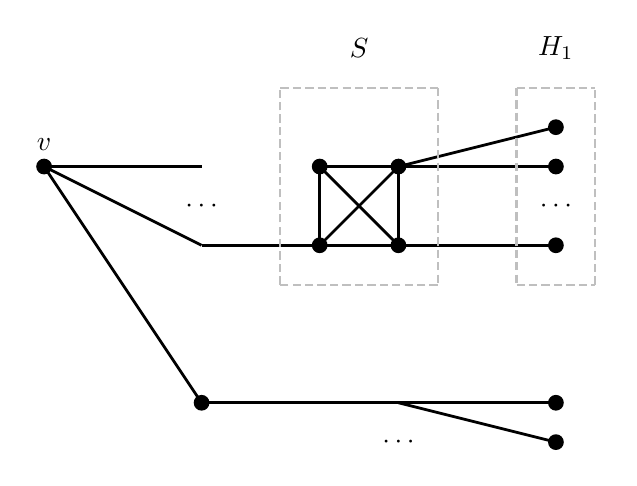
\begin{tikzpicture}
    \begin{pgfonlayer}{nodelayer}
        \node [label=above:{$v$}, BLACK_DOT] (1) at (-4.61111, 0.72222) {};
        \node [BLACK_DOT] (2) at (1.88889, 1.22222) {};
        \node [BLACK_DOT] (3) at (1.88889, 0.72222) {};
        \node [EMPTY] (4) at (1.88889, 0.22222) {$\cdots$};
        \node [BLACK_DOT] (5) at (1.88889, -0.27778) {};
        \node [BLACK_DOT] (6) at (1.88889, -2.27778) {};
        \node [BLACK_DOT] (7) at (1.88889, -2.77778) {};
        \node [BLACK_DOT] (8) at (-0.11111, 0.72222) {};
        \node [BLACK_DOT] (9) at (-1.11111, 0.72222) {};
        \node [BLACK_DOT] (10) at (-1.11111, -0.27778) {};
        \node [BLACK_DOT] (11) at (-0.11111, -0.27778) {};
        \node [EMPTY] (12) at (-2.61111, 0.72222) {};
        \node [EMPTY] (13) at (-2.61111, -0.27778) {};
        \node [EMPTY] (14) at (-2.61111, 0.22222) {$\cdots$};
        \node [EMPTY] (15) at (1.38889, 1.72222) {};
        \node [EMPTY] (16) at (1.38889, -0.77778) {};
        \node [EMPTY] (17) at (2.38889, -0.77778) {};
        \node [EMPTY] (18) at (2.38889, 1.72222) {};
        \node [EMPTY] (19) at (-1.61111, 1.72222) {};
        \node [EMPTY] (20) at (0.38889, -0.77778) {};
        \node [EMPTY] (21) at (-1.61111, -0.77778) {};
        \node [EMPTY] (22) at (0.38889, 1.72222) {};
        \node [BLACK_DOT] (23) at (-2.61111, -2.27778) {};
        \node [EMPTY] (24) at (-0.11111, -2.77778) {$\cdots$};
        \node [EMPTY] (25) at (-0.11111, -2.27778) {};
        \node [EMPTY] (26) at (1.88889, 2.22222) {$H_1$};
        \node [EMPTY] (27) at (-0.61111, 2.22222) {$S$};
    \end{pgfonlayer}
    \begin{pgfonlayer}{edgelayer}
        \draw[EDGE] (1) to (12);
        \draw[EDGE] (1) to (13);
        \draw[EDGE] (13) to (10);
        \draw[EDGE] (9) to (10);
        \draw[EDGE] (8) to (9);
        \draw[EDGE] (11) to (9);
        \draw[EDGE] (10) to (11);
        \draw[EDGE] (11) to (8);
        \draw[EDGE] (2) to (8);
        \draw[EDGE] (8) to (3);
        \draw[EDGE] (11) to (5);
        \draw[GRAY_DASHED_EDGE] (19) to (22);
        \draw[GRAY_DASHED_EDGE] (22) to (20);
        \draw[GRAY_DASHED_EDGE] (20) to (21);
        \draw[GRAY_DASHED_EDGE] (21) to (19);
        \draw[GRAY_DASHED_EDGE] (15) to (16);
        \draw[GRAY_DASHED_EDGE] (16) to (17);
        \draw[GRAY_DASHED_EDGE] (17) to (18);
        \draw[GRAY_DASHED_EDGE] (15) to (18);
        \draw[EDGE] (23) to (1);
        \draw[EDGE] (25) to (6);
        \draw[EDGE] (7) to (25);
        \draw[EDGE] (23) to (25);
        \draw[EDGE] (10) to (8);
    \end{pgfonlayer}
\end{tikzpicture}

\endgroup
		\caption{Demonstration of the proof of lemma \ref{lem:simplicial_vertex}. $H_1$ is a connected component of farthest vertices from $v$. $S$ is the set of vertices that are adjacent to $H_1$ and are not in $H_1$.
		}
		\label{fig:simplicial_vertex}
	\end{figure}
	I claim that $S$ is a clique.


	If $S$ contain only one vertex, there is nothing to prove.
	Assume $S$ contains at least two vertices. Let $u, w\in S$ be any distinct vertices.
	Both of $u, w$ are connected to $v$ via some vertices not in $H$, as they are closer to $v$. Both of them are also connected to some vertices in the connected component $H_1$.
	Note that no vertices in $H_1$ shall connected to any other vertices in closer to $v$ except those in $S$, as it will make the distance from $v$ to $H_1$ smaller.
	Therefore we are at the position to apply lemma \ref{lem:triangulated_cut_vertices} to the cycle formed by $u, w$ and any two vertices in $H_1$.
	In such way we have proved that any $u$ and $w \in S$ are adjacent, and therefore $S$ is a clique.

	Now apply the induction hypothesis to the subgraph induced by $H_1 \bigcup S$.
	If $H_1 \bigcup S$ is not a clique, then we can find a vertex $w \in H_1$ and $u \in S$ such that $w$ is distant 2 from $u$, and apply the induction hypothesis to the subgraph induced by $H_1 \bigcup S$ with $u$ as the chosen vertex states there is a simplicial vertex in $H_1$. 
	This vertex is also simplicial in $G$ as it is not adjacent to any vertices outside of $H_1 \bigcup S$.
	If $H_1 \bigcup S$ is a clique, then any vertex in $H_1$ is simplicial in $G$.
\end{proof}
